\chapter{معادلات حاکمه سیستم‌های ارتعاشی و فرمول‌بندی مسئله بهینه‌سازی}

\section{معادلات حاکمه سیستم‌های ارتعاشی}
\subsection{چارچوب عمومی و قابلیت تعمیم معادلات حاکم}

معادلات حاکم (\lr{Equations of Motion - EOM}) ارائه‌شده در این فصل بر پایه چارچوبی ریاضی جامع و قابل تعمیم استوار است که امکان مدل‌سازی و تحلیل سیستم‌های ارتعاشی پیچیده را با درجه آزادی بالا فراهم می‌آورد. این چارچوب از چهار اصل بنیادین زیر تبعیت می‌کند که عمومیت و کاربردی بودن آن را تضمین می‌کند:

\subsubsection{قابلیت تعمیم به سیستم‌های چنددرجه آزادی}
چارچوب ارائه‌شده به گونه‌ای طراحی شده که از سیستم‌های ساده تک‌درجه آزادی تا سیستم‌های پیچیده چنددرجه آزادی قابل گسترش است. این عمومیت از طریق فرمول‌بندی ماتریسی و بردار مختصات تعمیم‌یافته حاصل می‌شود که امکان مدل‌سازی برهم‌کنش‌های پیچیده بین اجزای مختلف سیستم را فراهم می‌آورد.

\subsubsection{ادغام المان‌های پیشرفته مکانیکی}
سیستم شامل تمامی المان‌های اساسی مکانیکی از جمله جرم‌ها، فنرها، میراگرها و \lr{Inerter}ها است که امکان مدل‌سازی رفتارهای دینامیکی متنوع را فراهم می‌آورد. این رویکرد با ادغام \lr{Inerter}ها که عناصری نوین در کنترل ارتعاش هستند، از رویکردهای سنتی فراتر می‌رود.

\subsubsection{سازگاری با روش‌های بهینه‌سازی پیشرفته}
معادلات حاکم به گونه‌ای فرمول‌بندی شده‌اند که به طور مستقیم با الگوریتم‌های بهینه‌سازی پیشرفته سازگار باشند. این اتصال امکان جستجوی کارآمد در فضای پارامتری بزرگ را فراهم می‌آورد و که در بخش های آتی به تفصیل بررسی خواهد شد.

\subsubsection{قابلیت پیاده‌سازی در نرم‌افزار تخصصی}
تمامی معادلات و روش‌های ارائه‌شده در این فصل در نرم‌افزار تخصصی \lr{DeVana} پیاده‌سازی شده‌اند که امکان تحلیل عددی، بهینه‌سازی و اعتبارسنجی نتایج را با رابط کاربری کاربرپسند فراهم می‌آورد و در فصل های آتی معرفی خواهد شد.

این رویکرد عمومی نه تنها برای سیستم‌های ارتعاشی خطی بلکه قابلیت گسترش به سیستم‌های غیرخطی را نیز دارا است و چارچوبی جامع برای حل مسائل بهینه‌سازی در مهندسی مکانیک فراهم می‌آورد.

\subsection{سیستم کاملاً کوپل شده \lr{2DOF-3DOF}}

\subsubsection{معماری سیستم و اجزای اصلی}
سیستم مورد بررسی یک سیستم پیشرفته کاملاً کوپل‌شده \lr{2DOF-3DOF} است که نماینده کلاس گسترده‌ای از سیستم‌های ارتعاشی چنددرجه آزادی در کاربردهای عملی مهندسی مکانیک می‌باشد. این سیستم از یک سازه اصلی دو درجه آزادی تشکیل شده که با سه جاذب ارتعاش دینامیکی تک‌درجه آزادی تقویت شده است.

\begin{figure}[H]
  \centering
  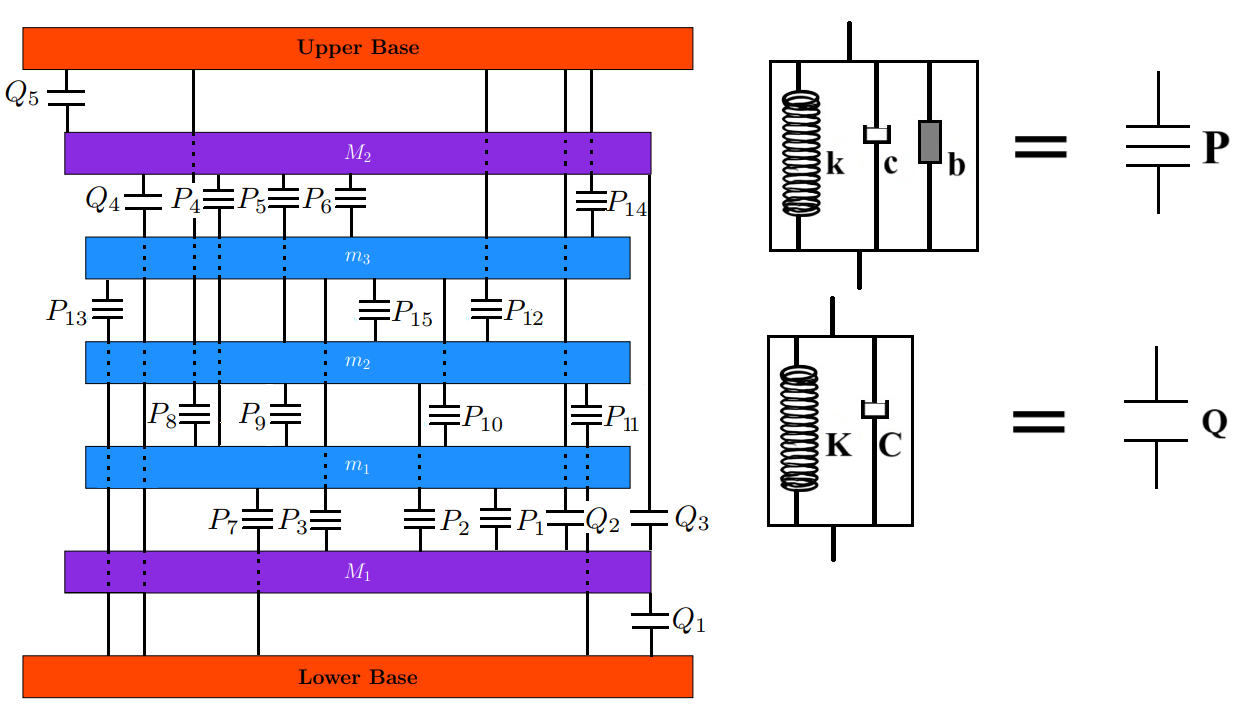
\includegraphics[width=\textwidth]{picture10.png}
  \caption{شماتیکی از سیستم کاملاً کوپل‌شده \lr{2DOF-3DOF}}\label{fig:2DOF-3DOF schematic}
\end{figure}

معماری سیستم شامل اجزای زیر است:
\begin{enumerate}
    \item \textbf{اجزای سازه‌ای اصلی}: دو جرم اصلی ($M_1$, $M_2$) نمایانگر اجزای سازه با خواص اینرسی
    \item \textbf{جاذب‌های ارتعاش دینامیکی}: سه جرم \lr{DVA} ($\mu_1$, $\mu_2$, $\mu_3$) با ویژگی‌های دینامیکی مستقل
    \item \textbf{تحریک‌های پایه}: حرکت پایه‌های پایین و بالا برای ورودی‌های ارتعاشی خارجی
    \item \textbf{نیروهای خارجی}: اعمال مستقیم نیرو بر جرم‌های اصلی
    \item \textbf{کوپلینگ کامل}: اتصال همه اجزا از طریق مؤلفه‌های جرمی، سختی، میرایی و اینرسی
\end{enumerate}

\subsubsection{فضای پارامتری و چالش‌های بهینه‌سازی}
سیستم دارای ۴۸ پارامتر طراحی مستقل است که به شرح زیر توزیع شده‌اند:
\begin{enumerate}
    \item ۱۵ پارامتر کوپلینگ جرمی ($\beta_1$ تا $\beta_{15}$) برای اتصالات اینرسی
    \item ۱۵ پارامتر سختی ($\lambda_1$ تا $\lambda_{15}$) برای کوپلینگ الاستیک
    \item ۱۵ پارامتر میرایی ($\nu_1$ تا $\nu_{15}$) برای اتلاف انرژی
    \item ۳ پارامتر جرم \lr{DVA} ($\mu_1$, $\mu_2$, $\mu_3$) برای تعیین اندازه جاذب‌ها
\end{enumerate}

این فضای پارامتری پیچیده نیازمند تکنیک‌های بهینه‌سازی پیشرفته است که بتوانند به طور کارآمد فضای طراحی را جستجو کنند.
\subsubsection{فرضیات مدل‌سازی و شرایط مرزی}
سیستم اصلی \lr{2DOF} با استفاده از چارچوبی جامع شامل جرم‌ها، فنرها، میراگرها و \lr{Inerter}ها مدل‌سازی می‌شود. رویکرد مدل‌سازی بر فرضیات بنیادی زیر استوار است:

\begin{enumerate}
    \item \textbf{رفتار الاستیک خطی}: تمام مؤلفه‌های سختی در بازه عملیاتی از رابطه نیرو-جابجایی خطی پیروی می‌کنند
    \item \textbf{میرایی ویسکوز خطی}: تمام مؤلفه‌های میرایی از روابط نیرو وابسته به سرعت خطی تبعیت می‌کنند
    \item \textbf{نمای جرم نقطه‌ای}: تمام جرم‌ها به صورت جرم نقطه‌ای با خواص اینرسی متمرکز در نظر گرفته می‌شوند
    \item \textbf{حرکت یک‌بعدی}: تمام مؤلفه‌های سیستم تنها در یک راستای انتقالی حرکت می‌کنند
    \item \textbf{پارامترهای ثابت در زمان}: همه پارامترهای سیستم در طول بهره‌برداری ثابت هستند
    \item \textbf{عدم وجود غیرخطی هندسی}: سیستم در ناحیه خطی عمل می‌کند
    \item \textbf{اتصال کامل و صلب}: همه اتصالات بین اجزا به صورت صلب فرض می‌شوند
\end{enumerate}

تحریک‌های پایه به گونه‌ای مدل‌سازی می‌شوند که سناریوهای مکانیکی مختلف را بازنمایی کنند. هر \lr{DVA} به صورت مستقل طراحی شده و کوپلینگ دینامیکی کامل از طریق مؤلفه‌های اتصال جامع تضمین می‌گردد.
\subsubsection{استخراج معادلات حاکم}
معادلات حاكم براي سيستم كاملاً كوپل‌شده \lr{2DOF-3DOF} با استفاده از روش نیوتن و با اعمال قانون دوم نیوتن بر هر درجه آزادي و در نظر گرفتن تمام نيروهاي اتصال‌دهنده استخراج مي‌شوند. مختصات تعميم‌يافته سيستم به صورت زير تعريف مي‌گردند:
\begin{align}\label{Eq.generalized.coordinate.2dof3dof}
    \mathbf{q} =
    \begin{bmatrix}
        U_1(t) \\
        U_2(t) \\
        u_1(t) \\
        u_2(t) \\
        u_3(t)
    \end{bmatrix}; \quad
    \dot{\mathbf{q}} =
    \begin{bmatrix}
        \dot{U_1}(t) \\
        \dot{U_2}(t) \\
        \dot{u_1}(t) \\
        \dot{u_2}(t) \\
        \dot{u_3}(t)
    \end{bmatrix}; \quad
    \ddot{\mathbf{q}} =
    \begin{bmatrix}
        \ddot{U_1}(t) \\
        \ddot{U_2}(t) \\
        \ddot{u_1}(t) \\
        \ddot{u_2}(t) \\
        \ddot{u_3}(t)
    \end{bmatrix}
\end{align}
كه در آن:
\begin{enumerate}
    \item $U_1(t)$، $U_2(t)$: جابجايي‌هاي جرم‌هاي اصلي در زمان $t$
    \item $u_1(t)$، $u_2(t)$، $u_3(t)$: جابجايي‌هاي جرم‌هاي \lr{DVA} در زمان $t$
\end{enumerate}
معادلات حركت به صورت ماتريسي بيان مي‌شوند:
\begin{equation} \label{Eq.EOM_dimensional_combined}
    \mathbf{M} \ddot{\mathbf{q}} + \mathbf{C} \dot{\mathbf{q}} + \mathbf{K} \mathbf{q} = \mathbf{F}(t)
\end{equation}
كه در آن: $\mathbf{q}$ بردار جابجايي‌هاي تعميم‌يافته است كه جابجايي جرم‌هاي اصلي و جرم‌هاي \lr{DVA} را دربر مي‌گيرد؛ $\mathbf{M}$ ماتريس جرم است؛ $\mathbf{C}$ ماتريس دمپينگ است؛ $\mathbf{K}$ ماتريس سختي است؛ و $\mathbf{F}(t)$ بردار نيروي خارجي است كه هم بارهاي خارجي و هم آثار حركت پايه را شامل مي‌شود.
بردار مختصات تعميم‌يافته به صورت زير بازتعريف مي‌شود:
\begin{equation}\label{Eq.generalized_coordinate_combined}
    \mathbf{q} = 
  \begin{bmatrix}
    U_1 \\ U_2 \\ u_1 \\ u_2 \\ u_3
  \end{bmatrix}
\end{equation}
\paragraph{ماتریس جرم}
\begin{equation}\label{Eq.mass_matrix_dimensional_combined}
\begin{aligned}
[M] =& 
\begin{bmatrix}
\shortstack[c]{$M_1 + b_1$ \\ $+ b_2 + b_3$} & 0 & \shortstack[c]{$-b_1$ \\ \,} & \shortstack[c]{$-b_2$ \\ \,} & \shortstack[c]{$-b_3$ \\ \,} \\
0 & \shortstack[c]{$M_2 + b_4$ \\ $+ b_5 + b_6$} & \shortstack[c]{$-b_4$ \\ \,} & \shortstack[c]{$-b_5$ \\ \,} & \shortstack[c]{$-b_6$ \\ \,} \\
\shortstack[c]{$-b_1$ \\ \,} & \shortstack[c]{$-b_4$ \\ \,} & \shortstack[c]{$m_1 + b_1$ \\ $+ b_4 + b_7$ \\ $+ b_8 + b_9$ \\ $+ b_{10}$} & \shortstack[c]{$-b_9$ \\ \,} & \shortstack[c]{$-b_{10}$ \\ \,} \\
\shortstack[c]{$-b_2$ \\ \,} & \shortstack[c]{$-b_5$ \\ \,} & \shortstack[c]{$-b_9$ \\ \,} & \shortstack[c]{$m_2 + b_2$ \\ $+ b_5 + b_9$ \\ $+ b_{11} + b_{12}$} & \shortstack[c]{$-b_{15}$ \\ \,} \\
\shortstack[c]{$-b_3$ \\ \,} & \shortstack[c]{$-b_6$ \\ \,} & \shortstack[c]{$-b_{10}$ \\ \,} & \shortstack[c]{$-b_{15}$ \\ \,} & \shortstack[c]{$m_3 + b_3$ \\ $+ b_6 + b_{10}$ \\ $+ b_{13} + b_{14}$ \\ $+ b_{15}$}
\end{bmatrix}
\end{aligned}
\end{equation}
 \noindent
\paragraph{ماتریس دمپینگ}
\begin{equation}\label{Eq.damping_matrix_dimensional_combined}
\begin{aligned}
[C] =& 
\begin{bmatrix}
\shortstack{$C_1 + C_2$ \\ $+ C_3$} & -C_3 & \shortstack{$-c_1$ \\ \,} & \shortstack{$-c_2$ \\ \,} & \shortstack{$-c_3$ \\ \,} \\
-C_3 & \shortstack{$C_3 + C_4$ \\ $+ C_5 + c_4$ \\ $+ c_5 + c_6$} & \shortstack{$-c_4$ \\ \,} & \shortstack{$-c_5$ \\ \,} & \shortstack{$-c_6$ \\ \,} \\
-c_1 & -c_2 & \shortstack{$c_1 + c_4$ \\ $+ c_7 + c_8$ \\ $+ c_9 + c_{10}$} & \shortstack{$-c_9$ \\ \,} & \shortstack{$-c_{10}$ \\ \,} \\
-c_2 & -c_5 & -c_9 & \shortstack{$c_2 + c_5$ \\ $+ c_9 + c_{11}$ \\ $+ c_{12} + c_{15}$} & \shortstack{$-c_{15}$ \\ \,} \\
-c_3 & -c_{6} & -c_{10} & -c_{15} & \shortstack{$c_3 + c_6$ \\ $+ c_{10} + c_{13}$ \\ $+ c_{14} + c_{15}$}
\end{bmatrix}
\end{aligned}
\end{equation}
\paragraph{ماتریس سختی}
\begin{equation}\label{Eq.stiffness_matrix_dimensional_combined}
\begin{aligned}
[K] =& 
\begin{bmatrix}
\shortstack{$K_1 + K_2$ \\ $+ K_3$} & -K_3 & \shortstack{$-k_1$ \\ \,} & \shortstack{$-k_2$ \\ \,} & \shortstack{$-k_3$ \\ \,} \\
-K_3 & \shortstack{$K_3 + K_4$ \\ $+ K_5 + k_4$ \\ $+ k_5 + k_6$} & \shortstack{$-k_4$ \\ \,} & \shortstack{$-k_5$ \\ \,} & \shortstack{$-k_6$ \\ \,} \\
-k_1 & -k_2 & \shortstack{$k_1 + k_4$ \\ $+ k_7 + k_8$ \\ $+ k_9 + k_{10}$} & \shortstack{$-k_9$ \\ \,} & \shortstack{$-k_{10}$ \\ \,} \\
-k_2 & -k_5 & -k_9 & \shortstack{$k_2 + k_5$ \\ $+ k_9 + k_{11}$ \\ $+ k_{12} + k_{15}$} & \shortstack{$-k_{15}$ \\ \,} \\
-k_3 & -k_{6} & -k_{10} & -k_{15} & \shortstack{$k_3 + k_6$ \\ $+ k_{10} + k_{13}$ \\ $+ k_{14} + k_{15}$}
\end{bmatrix}
\end{aligned}
\end{equation}
\paragraph{بردار نیرو}
\begin{equation}\label{Eq.force_vector_dimensional_combined}
\begin{aligned}
[F] = & \begin{bmatrix}
F_1(t) + C_1 \dot{U}_{low} + C_2 \dot{U}_{upp} + K_1 U_{low} + K_2 U_{upp} \\
F_2(t) + C_4 \dot{U}_{low} + C_5 \dot{U}_{upp} + K_4 U_{low} + K_5 U_{upp} \\
\beta_7 \ddot{U}_{low} + \beta_8 \ddot{U}_{upp} + 2 \zeta_{dc} \omega_{dc} (\nu_7 \dot{U}_{low} + \nu_8 \dot{U}_{upp}) + \omega_{dc}^2 (\lambda_7 U_{low} + \lambda_8 U_{upp}) \\
\beta_{11} \ddot{U}_{low} + \beta_{12} \ddot{U}_{upp} + 2 \zeta_{dc} \omega_{dc} (\nu_{11} \dot{U}_{low} + \nu_{12} \dot{U}_{upp}) + \omega_{dc}^2 (\lambda_{11} U_{low} + \lambda_{12} U_{upp}) \\
\beta_{13} \ddot{U}_{low} + \beta_{14} \ddot{U}_{upp} + 2 \zeta_{dc} \omega_{dc} (\nu_{13} \dot{U}_{low} + \nu_{14} \dot{U}_{upp}) + \omega_{dc}^2 (\lambda_{13} U_{low} + \lambda_{14} U_{upp})
\end{bmatrix}
\end{aligned}
\end{equation}
\subsubsection{صورت بی‌بعد}
به‌منظور ساده‌سازي تحليل، سيستم با استفاده از پارامترهاي بي‌بعدِ فهرست‌شده در جدول~\ref{Tab:dimensionless.table} نرمال‌سازي مي‌شود.
\begin{table}[h!]
\centering
\caption{پارامترهاي بي‌بعد براي نرمال‌سازي سيستم}
\label{Tab:dimensionless.table}
\begin{tabular}{lcc}
\toprule
\textbf{گروه پارامتر} & \textbf{پارامتر} & \textbf{تعريف} \\
\midrule
\textbf{نسبت‌هاي جرم} & \( \Gamma \) & \( \Gamma = \frac{M_2}{M_1} \) \\
 & \( \mu_i \) & \( \mu_i = \frac{m_i}{M_1} \) \\
\addlinespace
\textbf{نسبت‌هاي كوپلينگ اينرسي} & \( \beta_i \) & \( \beta_i = \frac{b_i}{M_1} \) \\
\addlinespace
\textbf{نسبت‌هاي دمپينگ} & \( \mathcal{N}_i \) & \( \mathcal{N}_i = \frac{C_i}{C_1} \) \\
 & \( \nu_i \) & \( \nu_i = \frac{c_i}{C_1} \) \\
\addlinespace
\textbf{نسبت‌هاي سختي} & \( \Lambda_i \) & \( \Lambda_i = \frac{K_i}{K_1} \) \\
 & \( \lambda_i \) & \( \lambda_i = \frac{k_i}{K_1} \) \\
\addlinespace
\textbf{سيستم اصليِ بدون كوپل} & \( \omega_{dc} \) & \( \omega_{dc} = \sqrt{\frac{K_1}{M_1}} \) \\
 & \( \zeta_{dc} \) & \( \zeta_{dc} = \frac{C_1}{2 M_1 \omega_{dc}} \) \\
\bottomrule
\end{tabular}
\end{table}
با استفاده از اين پارامترها، معادلات بي‌بعد حركت به صورت زير بيان مي‌شوند:
\begin{equation}\label{Eq.EOM_dimensionless}
\mathbf{\bar{M}} \ddot{\mathbf{q}} + 2 \zeta_{dc} \omega_{dc} \mathbf{\bar{C}} \dot{\mathbf{q}} + \omega_{dc}^2 \mathbf{\bar{K}} \mathbf{q} = \mathbf{\bar{F}}(t)
\end{equation}
ماتريس‌هاي بي‌بعد جرم، دمپينگ و سختي به همراه بردار نيرو در روابط \eqref{Eq.mass_matrix_dimensionless} تا \eqref{Eq.force_vector_dimensionless} تعريف مي‌شوند.
\paragraph{ماتریس جرم بی‌بعد}
\begin{equation}\label{Eq.mass_matrix_dimensionless}
\begin{aligned}
[\bar{M}] =& 
\begin{bmatrix}
\shortstack{$1 + \beta_1$ \\ $+ \beta_2 + \beta_3$} & 0 & \shortstack{$-\beta_1$ \\ \,} & \shortstack{$-\beta_2$ \\ \,} & \shortstack{$-\beta_3$ \\ \,} \\
0 & \shortstack{$\Gamma + \beta_4$ \\ $+ \beta_5 + \beta_6$} & \shortstack{$-\beta_4$ \\ \,} & \shortstack{$-\beta_5$ \\ \,} & \shortstack{$-\beta_6$ \\ \,} \\
-\beta_1 & -\beta_4 & \shortstack{$\mu_1 + \beta_1$ \\ $+ \beta_4 + \beta_7$ \\ $+ \beta_8 + \beta_9$ \\ $+ \beta_{10}$} & \shortstack{$-\beta_9$ \\ \,} & \shortstack{$-\beta_{10}$ \\ \,} \\
-\beta_2 & -\beta_5 & -\beta_9 & \shortstack{$\mu_2 + \beta_2$ \\ $+ \beta_5 + \beta_9$ \\ $+ \beta_{11} + \beta_{12}$} & \shortstack{$-\beta_{15}$ \\ \,} \\
-\beta_3 & -\beta_6 & -\beta_{10} & -\beta_{15} & \shortstack{$\mu_3 + \beta_3$ \\ $+ \beta_6 + \beta_{10}$ \\ $+ \beta_{13} + \beta_{14}$ \\ $+ \beta_{15}$}
\end{bmatrix}
\end{aligned}
\end{equation}
\paragraph{ماتریس دمپینگ بی‌بعد}
\begin{equation}\label{Eq.damping_matrix_dimensionless}
\begin{aligned}
[\bar{C}] =& 
\begin{bmatrix}
\shortstack{$1 + \mathcal{N}_2$ \\ $+ \mathcal{N}_3 + \nu_1$ \\ $+ \nu_2 + \nu_3$} & -\mathcal{N}_3 & \shortstack{$-\nu_1$ \\ \,} & \shortstack{$-\nu_2$ \\ \,} & \shortstack{$-\nu_3$ \\ \,} \\
-\mathcal{N}_3 & \shortstack{$\mathcal{N}_3 + \mathcal{N}_4$ \\ $+ \mathcal{N}_5 + \nu_4$ \\ $+ \nu_5 + \nu_6$} & \shortstack{$-\nu_4$ \\ \,} & \shortstack{$-\nu_5$ \\ \,} & \shortstack{$-\nu_6$ \\ \,} \\
-\nu_1 & -\nu_2 & \shortstack{$\nu_1 + \nu_4$ \\ $+ \nu_7 + \nu_8$ \\ $+ \nu_9 + \nu_{10}$} & \shortstack{$-\nu_9$ \\ \,} & \shortstack{$-\nu_{10}$ \\ \,} \\
-\nu_2 & -\nu_5 & -\nu_9 & \shortstack{$\nu_2 + \nu_5$ \\ $+ \nu_9 + \nu_{11}$ \\ $+ \nu_{12} + \nu_{15}$} & \shortstack{$-\nu_{15}$ \\ \,} \\
-\nu_3 & -\nu_{6} & -\nu_{10} & -\nu_{15} & \shortstack{$\nu_3 + \nu_6$ \\ $+ \nu_{10} + \nu_{13}$ \\ $+ \nu_{14} + \nu_{15}$}
\end{bmatrix}
\end{aligned}
\end{equation}
\paragraph{ماتریس سختی بی‌بعد}
\begin{equation}\label{Eq.stiffness_matrix_dimensionless}
\begin{aligned}
[\bar{K}] =& 
\begin{bmatrix}
\shortstack{$1 + \Lambda_2$ \\ $+ \Lambda_3 + \lambda_1$ \\ $+ \lambda_2 + \lambda_3$} & -\Lambda_3 & \shortstack{$-\lambda_1$ \\ \,} & \shortstack{$-\lambda_2$ \\ \,} & \shortstack{$-\lambda_3$ \\ \,} \\
-\Lambda_3 & \shortstack{$\Lambda_3 + \Lambda_4$ \\ $+ \Lambda_5 + \lambda_4$ \\ $+ \lambda_5 + \lambda_6$} & \shortstack{$-\lambda_4$ \\ \,} & \shortstack{$-\lambda_5$ \\ \,} & \shortstack{$-\lambda_6$ \\ \,} \\
-\lambda_1 & -\lambda_2 & \shortstack{$\lambda_1 + \lambda_4$ \\ $+ \lambda_7 + \lambda_8$ \\ $+ \lambda_9 + \lambda_{10}$} & \shortstack{$-\lambda_9$ \\ \,} & \shortstack{$-\lambda_{10}$ \\ \,} \\
-\lambda_2 & -\lambda_5 & -\lambda_9 & \shortstack{$\lambda_2 + \lambda_5$ \\ $+ \lambda_9 + \lambda_{11}$ \\ $+ \lambda_{12} + \lambda_{15}$} & \shortstack{$-\lambda_{15}$ \\ \,} \\
-\lambda_3 & -\lambda_{6} & -\lambda_{10} & -\lambda_{15} & \shortstack{$\lambda_3 + \lambda_6$ \\ $+ \lambda_{10} + \lambda_{13}$ \\ $+ \lambda_{14} + \lambda_{15}$}
\end{bmatrix}
\end{aligned}
\end{equation}
\paragraph{بردار نیروی بی‌بعد}
\begin{equation}\label{Eq.force_vector_dimensionless}
\begin{aligned}
[\bar{F}] = & \begin{bmatrix}
\frac{F_1(t)}{M_1} + 2 \zeta_{dc} \omega_{dc} (\dot{U}_{low} + \mathcal{N}_2 \dot{U}_{upp}) + \omega_{dc}^2 (U_{low} + \Lambda_2 U_{upp})\\
\frac{F_2(t)}{M_1} + 2 \zeta_{dc} \omega_{dc} (\mathcal{N}_4 \dot{U}_{low} + \mathcal{N}_5 \dot{U}_{upp}) + \omega_{dc}^2 (\Lambda_4 U_{low} + \Lambda_5 U_{upp}) \\
\beta_7 \ddot{U}_{low} +  \beta_8 \ddot{U}_{upp} +  2 \zeta_{dc} \omega_{dc} (\nu_7 \dot{U}_{low} + \nu_8 \dot{U}_{upp}) +\omega_{dc}^2 (\lambda_7 U_{low} + \lambda_8 U_{upp})\\
\beta_{11} \ddot{U}_{low} +  \beta_{12} \ddot{U}_{upp} +  2 \zeta_{dc} \omega_{dc} (\nu_{11} \dot{U}_{low} + \nu_{12} \dot{U}_{upp}) +\omega_{dc}^2 (\lambda_{11} U_{low} + \lambda_{12} U_{upp})\\
\beta_{13} \ddot{U}_{low} +  \beta_{14} \ddot{U}_{upp} +  2 \zeta_{dc} \omega_{dc} (\nu_{13} \dot{U}_{low} + \nu_{14} \dot{U}_{upp}) +\omega_{dc}^2 (\lambda_{13} U_{low} + \lambda_{14} U_{upp})
\end{bmatrix}
\end{aligned}
\end{equation}
\paragraph{راه‌حل‌های نیم تحلیلی برای تحریک هارمونیک}
روش نيم تحليلي بر تحريك هارمونيك و حركت هم‌فاز تكيه دارد. پاسخ سيستم به صورت زير بيان مي‌شود:
\begin{align}\label{Eq.harmonic.solution.2dof3dof}
    \begin{bmatrix}
        U_1(t) \\
        U_2(t) \\
        u_1(t) \\
        u_2(t) \\
        u_3(t)
    \end{bmatrix} =
    \begin{bmatrix}
        A_1 \\
        A_2 \\
        a_1 \\
        a_2 \\
        a_3
    \end{bmatrix} e^{j \omega t}
\end{align}
كه در آن $A_1, A_2$ دامنه ارتعاش جرم‌هاي اصلي و $a_1, a_2, a_3$ دامنه ارتعاش جرم‌هاي \lr{DVA} هستند.
تحريك‌هاي هارمونيك به صورت زير تعريف مي‌شوند:
\begin{align}\label{Eq.harmonic.excitations.2dof3dof}
    \begin{split}
        F_1(t) &= F_1 e^{j \omega t} \\
        F_2(t) &= F_2 e^{j \omega t} \\
        U_{Low}(t) &= A_{Low} e^{j \omega t} \\
        U_{Up}(t) &= A_{Up} e^{j \omega t}
    \end{split}
\end{align}
جايگزيني پاسخ‌هاي هارمونيك در معادلات حركت، فرمول‌بندي حوزه فركانس را نتيجه مي‌دهد:
\begin{align}\label{Eq.frequency.domain.2dof3dof}
    \begin{bmatrix}
        A_1 \\
        A_2 \\
        a_1 \\
        a_2 \\
        a_3
    \end{bmatrix} = \omega_{dc}^2 \left( -\Omega^2 \mathbf{M} + j 2 \zeta_{dc} \Omega \mathbf{C} + \mathbf{K} \right)^{-1} \mathbf{F}
\end{align}
كه در آن $\mathbf{F}$ بردار دامنه مختلط تابع نيرو است.
\subsection{مدل مرجع کاهش‌یافته \lr{1DOF-1DOF}}

\subsubsection{ضرورت استفاده از مدل کاهش‌یافته}
سیستم \lr{2DOF-3DOF} اصلی، با وجود جامعیت و قابلیت نمایش رفتارهای پیچیده، دارای چالش‌های اساسی در تحلیل پارامتری دقیق است. فضای پارامتری ۴۸-بعدی این سیستم، تحلیل تأثیر هر پارامتر به صورت ایزوله و تفکیک‌پذیر را دشوار می‌سازد. علاوه بر این، هزینه‌های محاسباتی بالا برای اجرای گسترده آزمون‌های پارامتری و تحلیل حساسیت، محدودیت‌هایی جدی در تفسیر نتایج ایجاد می‌کند.

برای غلبه بر این چالش‌ها، از یک مدل مرجع کاهش‌یافته \lr{1DOF-1DOF} استفاده می‌شود که امکان تحلیل دقیق‌تر و کارآمدتر پارامترهای طراحی را فراهم می‌آورد. این رویکرد در روش‌شناسی علمی به عنوان «مدل‌سازی سلسله‌مراتبی» شناخته می‌شود، جایی که ابتدا مفاهیم بنیادی در مدل‌های ساده‌تر بررسی شده و سپس به سیستم‌های پیچیده‌تر تعمیم داده می‌شود.

\subsubsection{معماری سیستم و ویژگی‌های طراحی}

سیستم \lr{1DOF-1DOF} مرجع به گونه‌ای طراحی شده که تمامی مکانیسم‌های اساسی کنترل ارتعاش را در خود جای دهد در حالی که پیچیدگی غیرضروری حذف شده است. این سیستم شامل سازه اصلی با یک درجه آزادی و جاذب دینامیکی با یک درجه آزادی است که هر دو به پایه‌های متحرک متصل هستند.

ویژگی‌های کلیدی این پیکربندی عبارتند از:
\begin{enumerate}
    \item \textbf{کوپلینگ کامل:} اتصال مستقیم بین سازه اصلی و جاذب از طریق عناصر مکانیکی، به علاوه اتصال هر دو به پایه متحرک
    \item \textbf{عناصر پیشرفته:} ادغام همزمان فنر، میراگر، و \lr{Inerter} برای نمایش کامل مکانیسم‌های کنترل ارتعاش
    \item \textbf{انعطاف‌پذیری پارامتری:} پارامترهای طراحی بهینه‌سازی‌شده شامل نسبت جرم، ضرایب سختی، میرایی، و پارامتر \lr{Inerter}
\end{enumerate}

\subsubsection{نقش در ارزیابی معیارهای عملکرد}

مدل کاهش‌یافته به عنوان سکوی آزمون ایده‌آلی برای ارزیابی و توسعه معیارهای عملکرد عمل می‌کند. به ویژه، امکان تحلیل دقیق معیار \lr{Peak-Slope (PS)} که هم دامنه قله و هم شیب اطراف آن را ارزیابی می‌کند، در این سیستم فراهم است. این ارزیابی جامع تضمین می‌کند که طراحی‌های بهینه نه تنها حداکثر ارتعاش را کاهش می‌دهند، بلکه پایداری پاسخ در حوالی رزونانس را نیز بهبود می‌بخشند.

به این ترتیب، سیستم \lr{1DOF-1DOF} پلی میان مفاهیم نظری و کاربردهای عملی ایجاد می‌کند و امکان انتقال دانش از مدل ساده به سیستم‌های پیچیده را فراهم می‌آورد.
\begin{figure}[H]
\centering
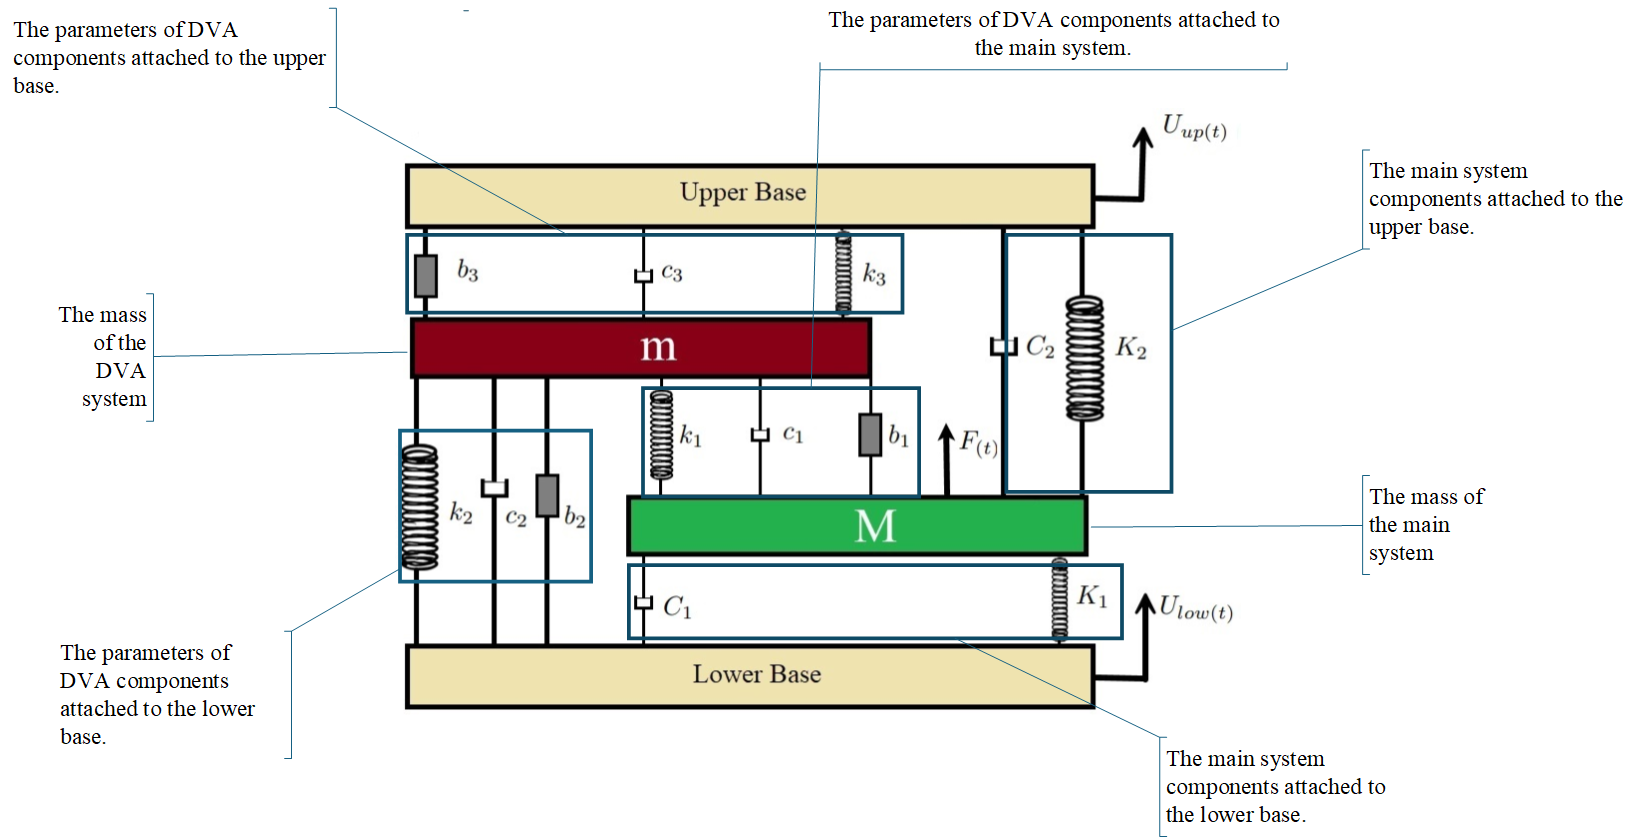
\includegraphics[width=1.1\textwidth]{picture3.png}
\caption{نمای شماتیک از یک سیستم کاملاً کوپل‌شده \lr{1DOF–1DOF} (مدل کاهش‌یافته مرجع)}
\label{fig:fully-coupled-1dof}
\end{figure}

\section{فرمول‌بندی مسئله بهینه‌سازی}
\subsection{تعریف مسئله بهینه‌سازی}
با اتکا به سيستم مكانيكي پيچيده \lr{2DOF-3DOF} توصيف‌شده در بخش پيش، مسئله بهينه‌سازي به‌گونه‌اي فرموله مي‌شود كه پارامترهاي بهينهِ جاذب دینامیکی ارتعاشات\lr{(DVA)} را براي كاهش انحراف از ويژگي‌هاي عملكردي مطلوب سامانه بيابد. سامانه شامل ۴۸ پارامتر طراحي مستقل است كه در ميان ۱۵ ضريب كوپلينگ جرمي ($\beta_1$ تا $\beta_{15}$)، ۱۵ پارامتر سختي ($\lambda_1$ تا $\lambda_{15}$)، ۱۵ پارامتر دمپينگ ($\nu_1$ تا $\nu_{15}$)، و ۳ پارامتر جرم \lr{DVA} ($\mu_1$, $\mu_2$, $\mu_3$) توزيع شده‌اند.
مسئله بهينه‌سازي به صورت زير بيان رياضي مي‌شود:
\begin{equation}\label{Eq.optimization_problem}
\begin{aligned}
\min_{\mathbf{x}} \quad & f(\mathbf{x}) = f_{primary}(\mathbf{x}) + f_{sparsity}(\mathbf{x}) + f_{error}(\mathbf{x}) \\
\mtext{subject to} \quad & \mathbf{x}_L \leq \mathbf{x} \leq \mathbf{x}_U \\
\end{aligned}
\end{equation}
كه در آن:
\begin{enumerate}
    \item $\mathbf{x} \in \mathbb{R}^{48}$ بردار پارامترهاي طراحي است
    \item $\mathbf{x}_L, \mathbf{x}_U \in \mathbb{R}^{48}$ به‌ترتيب كف و سقف مجاز پارامترها هستند
    \item $f_{primary}(\mathbf{x})$، $f_{sparsity}(\mathbf{x})$، $f_{error}(\mathbf{x})$ مؤلفه‌هاي تابع هدف هستند
\end{enumerate}

\subsection{تعریف تابع هدف}
تابع هدف كل، جمعِ وزنيِ سه مؤلفه متمايز است كه هر يك به جنبه‌اي از مسئله بهينه‌سازي می پردازند :
\begin{equation}\label{Eq.objective_function_detailed}
f(\mathbf{x}) = f_{primary}(\mathbf{x}) + f_{sparsity}(\mathbf{x}) + f_{error}(\mathbf{x})
\end{equation}
كه در آن هر مؤلفه به‌صورت دقيق تعريف شده و نقش مشخصي در فرآيند بهينه‌سازي ايفا مي‌كند.
\textbf{تابع هدف اصلي ($f_{primary}(\mathbf{x})$):} اين مؤلفه، انحراف پاسخ تكين سامانه از مقدار هدف $1.0$ را اندازه‌گيري مي‌كند:
\begin{equation}\label{Eq.primary_objective_detailed}
f_{primary}(\mathbf{x}) = \left| C_s(\mathbf{x}) - 1.0 \right|
\end{equation}
كه در آن معيار تكين $C_s(\mathbf{x})$ به صورت زير محاسبه مي‌شود:
\begin{equation}\label{Eq.singular_response_detailed}
C_s(\mathbf{x}) = \sum_{i=1}^{5} CM_i(\mathbf{x})
\end{equation}
و $CM_i(\mathbf{x})$ «معيار تركيبي» براي جرمِ $i$ام است:
\begin{equation}\label{Eq.composite_measure_detailed}
CM_i(\mathbf{x}) = \sum_{j} w_{ij} \cdot \frac{a_{ij}(\mathbf{x})}{t_{ij}}
\end{equation}
معيار تركيبي چندين شاخص عملكردي را براي هر جرم يكپارچه مي‌كند؛ به‌طوري‌كه:
\begin{enumerate}
    \item $w_{ij}$: ضريب وزن براي شاخصِ $j$امِ جرمِ $i$ام
    \item $a_{ij}(\mathbf{x})$: مقدار عملكرديِ مشاهده‌شده براي شاخصِ $j$امِ جرمِ $i$ام
    \item $t_{ij}$: مقدار هدف براي شاخصِ $j$امِ جرمِ $i$ام
\end{enumerate}
شاخص‌هاي عملكردي شامل مكانِ قله‌ها، مقدار قله‌ها، پهناي باند، شيب‌ها و مساحت زير منحني (استخراج‌شده از تحليل \lr{FRF}) هستند. ضرائب وزن امكان اولويت‌بنديِ جنبه‌هاي مختلف عملكرد را فراهم مي‌كنند و معمولاً برحسب اهميت هر شاخص، در بازه‌اي حدود $0.05 $تا $1.0$ انتخاب مي‌شوند.
\textbf{تابع جريمهِ تنكي ($f_{sparsity}(\mathbf{x})$):} اين مؤلفه، پاسخ هایی که باکمترین تعداد پارامتر های \lr{DVA} می باشد را ارجعیت قرار میدهد:
\begin{equation}\label{Eq.sparsity_penalty_detailed}
f_{sparsity}(\mathbf{x}) = \alpha \sum_{k=1}^{48} |x_k|
\end{equation}
كه در آن:
\begin{enumerate}
    \item $\alpha$ ضريب وزن تنكي است
    \item $x_k$ نمايانگر پارامتر طراحيِ $k$ام است
    \item به‌كارگيري منظم‌سازي \lr{L1} با جريمه‌كردنِ مقادير ناصفر، راهكارهاي تنك را ترويج مي‌كند
\end{enumerate}
اين تابع چند هدف كاربردي را دنبال مي‌كند:
\begin{enumerate}
    \item \textbf{منظم‌سازي}: از بيش‌برازش نسبت به بازه‌هاي فركانسي خاص جلوگيري مي‌كند و از تركيب‌هاي بسيار پيچيده پارامترها پرهيز مي‌شود
    \item \textbf{پياده‌سازي عملي}: به پيكربندي‌هاي ساده‌تر \lr{DVA} كه ساخت و نگهداري آن‌ها آسان‌تر است انگيزه مي‌دهد
    \item \textbf{افزايش پايايي}: حساسيت نسبت به تغييرات پارامتر در كاربردهاي واقعي را كاهش مي‌دهد
\end{enumerate}
\textbf{مؤلفه خطاي درصدي ($f_{error}(\mathbf{x})$):} اين مؤلفه، انحراف‌هاي عملكرديِ جزئي را به‌صورت دقيق در بر مي‌گيرد:
\begin{align}\label{Eq.percentage_error_detailed}
f_{error}(\mathbf{x}) &= \frac{1}{\gamma} \sum_{i} \sum_{j} \left| PD_{ij}(\mathbf{x}) \right|\\
PD_{ij}(\mathbf{x}) &= \left( \frac{a_{ij}(\mathbf{x}) - t_{ij}}{|t_{ij}|} \right) \times 100\%
\end{align}
كه در آن، $\gamma$ ضريب مقياس‌گذاري (با مقدار پيش‌فرض 1000) است و $PD_{ij}(\mathbf{x})$ اختلافِ درصدي براي شاخصِ $j$امِ جرمِ $i$ام را نشان مي‌دهد؛ همچنين استفاده از قدرمطلق مانع از خنثي‌شدن خطاهاي مثبت و منفي مي‌شود. اين مؤلفه تضمين مي‌كند كه ارزيابي به‌صورت جامع انجام شود، زيرا تمام انحراف‌هاي شاخص‌هاي عملكردي را در تابع هدف پوشش مي‌دهد و امكان لحاظ هم‌زمان ويژگي‌هاي كلي پاسخ و سنجه‌هاي جزئيِ عملكرد را فراهم مي‌سازد. همچنين، با تعيين مقادير هدف براي شاخص‌ها، تفاوت در اهميت آن‌ها را مجاز مي‌داند و معياري نرمال‌شده از خطا ارائه مي‌دهد كه قابل مقايسه ميان انواع مختلف شاخص‌ها است. در نهايت، ضريب مقياس $\gamma$ نقش موازنه‌كننده سهم سنجه‌هاي جزئي با تابع هدف اصلي را ايفا مي‌كند.
ضريب مقياس $\gamma$ نقشي كليدي در ترازكردن سهم مؤلفه خطاي درصدي نسبت به ساير مؤلفه‌هاي هدف دارد؛ انتخابِ $\gamma$ بزرگ‌تر، تأثير خطاهاي درصديِ جزئي را كاهش مي‌دهد و انتخابِ $\gamma$ كوچك‌تر، اهميت آن‌ها را در بهينه‌سازي كل افزايش مي‌دهد.

\textbf{محاسبات سنجه‌های عملکرد:} پاسخ هر جرم تحت یک تحلیل جامع قرار می‌گیرد:

\begin{enumerate}
    \item \textbf{تحلیل مقدار قله در پاسخ فرکانسی (\lr{Y-Value}):}
    \begin{equation}\label{Eq.peak_amplitude_analysis_detailed}
    A_{peak,i} = \max_{j} |X_i(\omega_j)| \quad \forall i = 1,\ldots,5
    \end{equation}

    \item \textbf{تحلیل فرکانس متناظر با قله (\lr{X-Value}):}
    \begin{equation}\label{Eq.peak_frequency_analysis_detailed}
    \omega_{peak,i} = \omega_{j^*} \quad \text{که در آن} \quad j^* = \arg\max_{j} |X_i(\omega_j)|, \quad \forall i = 1,\ldots,5
    \end{equation}

    \item \textbf{تحلیل پهنای‌باند بر اساس تابع انتقال فرکانسی (\lr{FRF}) برای یک جرم معین $i$:}
    برای هر جرم $i$، پهنای‌باند به عنوان فاصله فرکانسی بین دو قله اصلی (دو مود غالب) در پاسخ فرکانسی همان جرم تعریف می‌شود. این دو قله با اندیس‌های $j$ و $k$ (که $j < k$) مشخص می‌شوند و از روی نمودار \lr{FRF} یعنی $|X_i(\omega)|$ استخراج می‌گردند:
    \begin{equation}\label{Eq.bandwidth_analysis_detailed}
    \Delta\omega_{i,(j,k)} = |\omega_{peak,i,k} - \omega_{peak,i,j}| \quad \forall j < k
    \end{equation}
    که در آن $\omega_{peak,i,j}$ و $\omega_{peak,i,k}$ به ترتیب فرکانس‌هایی هستند که در آن‌ها $|X_i(\omega)|$ به دو بیشینه محلی خود (دو قله اصلی) می‌رسد. این شاخص فاصله بین دو مود غالب جرم $i$ را در \lr{FRF} نشان می‌دهد و برای ارزیابی جداسازی مودها و کنترل رفتار دینامیکی همان جرم اهمیت دارد.

    \item \textbf{تحلیل معیار شیب-قله:}
    شیب بین دو قله اصلی در نمودار \lr{FRF} برای جرم $i$ام و بین دو قله $j$ام و $k$ام (که $j < k$) به صورت زیر تعریف می‌شود:
    \begin{equation}\label{Eq.slope_analysis_detailed}
    s_{i,(j,k)} = \frac{A_{peak,i,k} - A_{peak,i,j}}{\omega_{peak,i,k} - \omega_{peak,i,j}} \quad \forall j < k
    \end{equation}
    که در آن $A_{peak,i,j} = |X_i(\omega_{peak,i,j})|$ و $A_{peak,i,k} = |X_i(\omega_{peak,i,k})|$ هستند. این شاخص نرخ تغییر دامنه پاسخ فرکانسی جرم $i$ام بین دو مود غالب $j$ام و $k$ام را نشان می‌دهد و از روی شیب منحنی \lr{FRF} بین این دو قله محاسبه می‌شود. 

    \item \textbf{تحلیل مساحت زیر منحنی \lr{FRF}:}
    مساحت زیر منحنی پاسخ فرکانسی برای هر جرم $i$ (\lr{$i=1,\ldots,5$}) به صورت انتگرال مقدار مطلق \lr{FRF} در بازه فرکانسی مورد نظر تعریف می‌شود:
    \begin{equation}\label{Eq.area_analysis_detailed}
    Area_i = \int_{\omega_{start}}^{\omega_{end}} |X_i(\omega)| \, d\omega \qquad (i=1,\ldots,5)
    \end{equation}
    این شاخص بیانگر انرژی کل منتقل‌شده به جرم $i$ در بازه فرکانسی است و به طور مستقیم از روی نمودار \lr{FRF} محاسبه می‌شود. مقدار کمتر این مساحت معمولاً به معنای کنترل بهتر ارتعاشات و عملکرد مطلوب‌تر جاذب‌ها است.

\end{enumerate}
انتگرال مساحت برای دقت عددی با استفاده از قاعده \lr{Simpson} محاسبه می‌شود:
\begin{equation}\label{Eq.area_simpson_detailed}
Area_i \approx \frac{h}{3} \left[ |X_i(\omega_0)| + 4\sum_{k=1}^{n/2} |X_i(\omega_{2k-1})| + 2\sum_{k=1}^{n/2-1} |X_i(\omega_{2k})| + |X_i(\omega_n)| \right]
\end{equation}
که در آن $h$ گام فرکانسی و $n$ تعداد نقاط فرکانسی است.

\section{پیوند با روش‌های بهینه‌سازی و پیاده‌سازی}

\subsection{سازگاری با الگوریتم ژنتیک پیشرفته}
معادلات حاکم ارائه‌شده در این فصل، بنیادی محکم برای اعمال روش‌های بهینه‌سازی پیشرفته فراهم می‌آورد. این معادلات به طور مستقیم با الگوریتم ژنتیک (\lr{GA}) سازگار هستند که امکان جستجوی کارآمد در فضای پارامتری پیچیده سیستم را فراهم می‌آورد و در فصل چهارم به تفصیل بررسی خواهد شد.

\subsection{پیاده‌سازی در نرم‌افزار DeVana}
تمامی معادلات حاکم و روش‌های ارائه‌شده در این فصل در نرم‌افزار تخصصی \lr{DeVana} پیاده‌سازی شده‌اند. این نرم‌افزار امکان تحلیل عددی، بهینه‌سازی و اعتبارسنجی نتایج را با رابط کاربری کاربرپسند فراهم می‌آورد و در فصل ششم معرفی خواهد شد.

\subsection{اهمیت عمومیت رویکرد ارائه‌شده}
چارچوب ریاضی ارائه‌شده فراتر از سیستم خاص \lr{2DOF-3DOF} است و قابلیت تعمیم به کلاس گسترده‌ای از سیستم‌های ارتعاشی را دارا است. این عمومیت از طریق فرمول‌بندی ماتریسی، پارامتری‌سازی بی‌بعد، ادغام المان‌های پیشرفته و سازگاری با روش‌های عددی حاصل می‌شود.


